%----------------------------------------------------------------------------
%----------------------------------------------------------------------------
%----------------------------------------------------------------------------
Suppose the dynamics of some three level quantum system is given by
%----------------------------------------------------------------------------
\begin{equation}
i\frac{\partial}{\partial t} \ket{\Psi}
=
i\left(
\begin{array}{cccc}
0 & \alpha & 0 \\
-\alpha & 0 & \beta \\
0 & -\beta & 0
\end{array}
\right)
\ket{\Psi},
\label{two dynamics}
\end{equation}
%----------------------------------------------------------------------------
where the square of the nth element in $\ket{\Psi}$ is the probability of finding the system in the nth state, $\alpha$ is the coupling field between the zeroth (ground) and first state and $\beta$ is the coupling field between the first and second state. Using the same methods as in Section \ref{basic_two_level}, it can be shown that closed non-degenerate three level quantum systems with two completely resonant ``ladder'' coupling fields can be described this way in the energy basis (see Figure \ref{2 color ladder}).
%----------------------------------------------------------------------------
%----------------------------------------------------------------------------
% 2_color_ladder.tex
% by Troy Hix, March 2005
%----------------------------------------------------------------------------
%----------------------------------------------------------------------------
\begin{figure}
\setlength{\unitlength}{2cm}
\begin{center}
\begin{picture}(3.3,2.2)
\linethickness{1mm}
\put(0,2.0){\line(1,0){3}}
\put(0,1.2){\line(1,0){3}}
\put(0,0.0){\line(1,0){3}}
\put(3.1,2.0){$\ket{2}$}
\put(3.1,1.2){$\ket{1}$}
\put(3.1,0.0){$\ket{0}$}
\thinlines
\put(1.0,1.2){\vector(0,1){0.78}}
\put(1.0,0.0){\vector(0,1){1.18}}
\put(1.2,1.6){$\beta$}
\put(1.2,0.6){$\alpha$}
\end{picture}
\end{center}
\caption[Three level, two field diagram]{Three level, two field diagram. Ground state $\ket{0}$, first excited state $\ket{1}$, and second excited state $\ket{2}$ are coupled by fields $\alpha$ and $\beta$ so that population transfers from the ground state to the second excited state}
\label{2 color ladder}
\end{figure}
%----------------------------------------------------------------------------
%----------------------------------------------------------------------------

%----------------------------------------------------------------------------
%----------------------------------------------------------------------------
%----------------------------------------------------------------------------
%----------------------------------------------------------------------------
Again, we consider temporally localized coupling fields of the form given in equation (\ref{gaussian}) for $\alpha$ and similarly for $\beta$. Let the position of $\alpha$ be given in terms of $\beta$'s position; namely let $\Delta_\alpha$ be the temporal distance alpha \emph{leads} beta; specifically
%----------------------------------------------------------------------------
\begin{subequations}
\begin{eqnarray} 
t_\alpha & = & t_0 - \frac{\Delta_\alpha}{2} \\
t_\beta  & = & t_0 + \frac{\Delta_\alpha}{2}
\end{eqnarray}
\label{temporal position}
\end{subequations}
%----------------------------------------------------------------------------
where $t_0$ is the center of the pulse sequence. For example, in the sequential order shown in Figure \ref{2_pulses}, $\Delta_\alpha$ is positive.
%----------------------------------------------------------------------------
%----------------------------------------------------------------------------
% 2_pulses.tex
% by Troy Hix, March 2005
%----------------------------------------------------------------------------
\begin{figure}
\centering
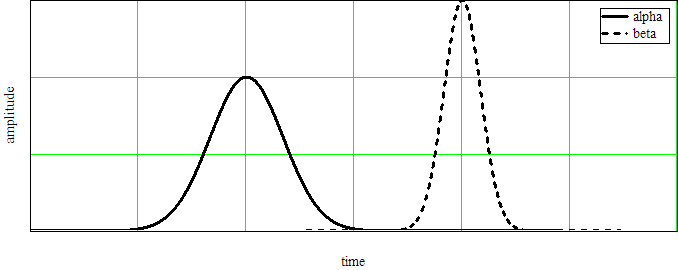
\includegraphics[width=5.00in]
{2_pulses/2_pulses.png}\\
\caption[Two pulse sequence example]{Two pulse sequence example. In general the pulses $\alpha$ and $\beta$ have arbitrary widths $\sigma_\alpha$ and  $\sigma_\beta$ as well as arbitrary amplitudes $A$ and $B$. Here $\Delta_\alpha$ is positive since $\alpha$ precedes $\beta$.}
\label{2_pulses}
\end{figure} 
%----------------------------------------------------------------------------

%----------------------------------------------------------------------------
%----------------------------------------------------------------------------
